\chapter{Approach}\label{chapter:approach}

\pgfplotstableread[col sep=comma]{data/sys_lit_rev.csv}\mytable

\def\printonlypositive#1{\ifnum#1>0
#1
\fi}

This thesis aims to identify the most widely used frameworks for generating synthetic \textit{Zipfian} distributed data in the systems programming and database community and 
make a comparative evaluation.
The first step required to achieve this is a systematic review of current approaches. The following sections describe
\begin{enumerate}
    \item The \textbf{research approach} used to identify the frameworks
    \item The \textbf{common frameworks} recognized from the search along with short descriptions
    \item The \textbf{popularity and impact} of those tools
    \item The \textbf{benchmarking module} which will be used to evaluate the frameworks
\end{enumerate}

\section{Research Approach}
First, a list of relevant conferences and journals was defined to identify frameworks the systems programming and database community used.
 The six following conferences were taken into account:
\begin{center} 
    \begin{minipage}{0.8\linewidth} 
      \begin{multicols}{2} 
        \begin{itemize}
          \raggedright
          \item \ac{PVLDB}
          \item \ac{SIGMOD}
          \item \ac{CIDR}
          \item \ac{OSDI}
          \item \ac{NSDI}
          \item \ac{FAST}
        \end{itemize}
      \end{multicols}
      \label{list:conferences}
    \end{minipage}
\end{center}

These conferences were chosen due to their high selectivity and special relevancy for storage technology research, where standardized IO benchmarks are prevalent
. The search was conducted broadly following the steps indicated in \parencite{bramerSystematicApproachSearching2018}, as defined below: 
\begin{enumerate}
    \item Word search on keyword search matrix (see table~\ref{tab:keyword_search_matrix})
    \item Identify the frameworks used in the papers
    \item Extended keyword search, this time adding the frameworks identified in the previous step
\end{enumerate} 

The first step suggests the use of a \textit{keyword matrix}. Such a matrix can be built by choosing appropriate keywords
that refer to the topic of interest, so all words should be present in the works searched. 
Synonyms are used to improve the accuracy and scope of the search. It is defined as follows:

\begin{table}[h!]
    \centering
    \begin{tabular}{|c|l|r|r|}
      \hline
       & \multicolumn{1}{c|}{Keyword 1} & \multicolumn{1}{c|}{Keyword 2} & \multicolumn{1}{c|}{Keyword 3} \\ \hline
       \parbox[t]{4mm}{\multirow{3}{*}{\rotatebox[origin=r]{90}{synonyms}}}
       & zipf   &   benchmark     &    synthetic      \\
       & zipfian   &   workload     &    generated      \\
       &    &   evaluation     &    sampled      \\
       &    &   empirical     &    sampler      \\
       &   &   dataset     &         \\ \hline
    \end{tabular}
    \caption{Keyword search matrix}
    \label{tab:keyword_search_matrix}
  \end{table} 

Given this matrix, the search was conducted on the following academic databases: \textit{IEEE Xplore}, \textit{ACM Digital Library}, \textit{DBLP}, and \textit{Google Scholar}. 
The results were sorted in \textit{relevance} order, such that well-cited but also relatively new papers appear at the top. An analysis of the findings follows in the next section.

\section{Common Frameworks}

In the first phase, the following frameworks were identified among the top 20 results of each conference
\begin{center}
    \begin{tabular}{|l|}
        \hline
        \textbf{Frameworks} \\ \hline\hline
        \ac{YCSB} \cite{cooperBenchmarkingCloudServing2010} \\ \hline
        \ac{FIO} \cite{1FioFlexible} \\ \hline
        Sysbench \cite{kopytovAkopytovSysbench2025} \\ \hline
        OLTP-Bench \cite{difallahOLTPBenchExtensibleTestbed2013} \\ \hline
    \end{tabular}
\end{center}

The previous keyword matrix was extended with the frameworks' names to assert their popularity in the six venues. 
Pie charts in Figure \ref{fig:popularity_frameworks} show the trends found.

\begin{figure}[h]
    \centering
    \def\printonlypositive#1{\ifnum#1>0
#1
\fi}

\begin{tikzpicture}

% Pie #1: PVLDB
\begin{scope}[xshift=0cm,yshift=0cm]
  \node[font=\bfseries] at (0,1.8){PVLDB};
  \pie[
    sum=auto,
    radius=1.3,
    text=,
    before number=\printonlypositive,
    color={blue!50!white, red!50!white, green!50!white, orange!50!white}
  ]{
    109/YCSB,
    3/Sysbench,
    3/FIO,
    8/OLTPBench
  }
\end{scope}

% Pie #2: SIGMOD
\begin{scope}[xshift=4cm,yshift=0cm]
  \node[font=\bfseries] at (0,1.8){SIGMOD};
  \pie[
    sum=auto,
    radius=1.3,
    text=,
    before number=\printonlypositive,
    color={blue!50!white, red!50!white, green!50!white, orange!50!white}
  ]{
    18/YCSB,
    2/Sysbench,
    0/FIO,
    2/OLTPBench
  }
\end{scope}

% Pie #3: CIDR
\begin{scope}[xshift=8cm,yshift=0cm]
  \node[font=\bfseries] at (0,1.8){CIDR};
  \pie[
    sum=auto,
    radius=1.3,
    text=,
    before number=\printonlypositive,
    color={blue!50!white, red!50!white, green!50!white, orange!50!white}
  ]{
    4/YCSB,
    0/Sysbench,
    1/FIO,
    1/OLTPBench
  }
\end{scope}

% Pie #4: FAST
\begin{scope}[xshift=0cm,yshift=-4cm]
  \node[font=\bfseries] at (0,1.8){FAST};
  \pie[
    sum=auto,
    radius=1.3,
    text=,
    before number=\printonlypositive,
    color={blue!50!white, red!50!white, green!50!white, orange!50!white}
  ]{
    35/YCSB,
    0/Sysbench,
    3/FIO,
    2/OLTPBench
  }
\end{scope}

% Pie #5: NSDI
\begin{scope}[xshift=4cm,yshift=-4cm]
  \node[font=\bfseries] at (0,1.8){NSDI};
  \pie[
    sum=auto,
    radius=1.3,
    text=,
    before number=\printonlypositive,
    color={blue!50!white, red!50!white, green!50!white, orange!50!white}
  ]{
    24/YCSB,
    0/Sysbench,
    0/FIO,
    0/OLTPBench
  }
\end{scope}

% Pie #6: OSDI
\begin{scope}[xshift=8cm,yshift=-4cm]
  \node[font=\bfseries] at (0,1.8){OSDI};
  \pie[
    sum=auto,
    radius=1.3,
    text=legend,
    before number=\printonlypositive,
    color={blue!50!white, red!50!white, green!50!white, orange!50!white}
  ]{
    26/YCSB,
    0/Sysbench,
    3/FIO,
    0/OLTPBench
  }
\end{scope}

\end{tikzpicture}
    \caption{Popularity of the frameworks in the conferences}
    \label{fig:popularity_frameworks}
\end{figure}

The most popular framework is \textbf{YCSB}, followed by \textbf{OLTPBench}, as well as \textbf{FIO}. Although this would point to a clear winner in \textbf{YCSB}, 
it is important to note that the popularity of a framework considered in academic journals might not reflect its actual usage in practice. 
A search for the frameworks in \textit{GitHub} yielded the table \ref{fig:popularity_frameworks} (as of 22 March 2025), containing
the number of \textit{starts} given to a code repository. 

\begin{table}[h]
    \centering
    \begin{tabular}{|l|r|}
      \hline
      \textbf{Framework} & \textbf{Stars} \\ \hline\hline
      YCSB & 5k \\ \hline
      Sysbench & 6.3k \\ \hline
      FIO & 5.5k \\ \hline
      OLTPBench & 0.5k \\ \hline
    \end{tabular}
    \caption{Popularity of the frameworks on GitHub}
    \label{tab:popularity_github}
\end{table}

\subsection{Yahoo! Cloud Serving Benchmark}
\ac{YCSB} is a widely used benchmarking tool for cloud databases, developed by \textit{Yahoo! Research} and now maintained by a community of developers. 
The framework generates \textit{workloads} used to test the performance of database systems under stress, by populating tables with entries. How these entries are distributed
is not fixed and can be chosen by the user. One of the possible distributions is the \textit{Zipfian}, and a submodule in \ac{YCSB} is responsible for generating variates.

In order to compute the samples, the benchmark suite uses the algorithm proposed by Gray, as presented before (see \ref{subsec:jim_gray}). One limiting factor in his original paper
 is that generated keys are lexicographically sorted, e.g. key $0$ has the highest frequency. 
 The keys should be randomly distributed within the support distribution to better reflect real workloads.
See Figure \ref{fig:zipfian_comparison_ycsb} for a comparison of these two cases.

% TODO : Fix x,y-axis labels 
\begin{figure}[h]
    \centering
    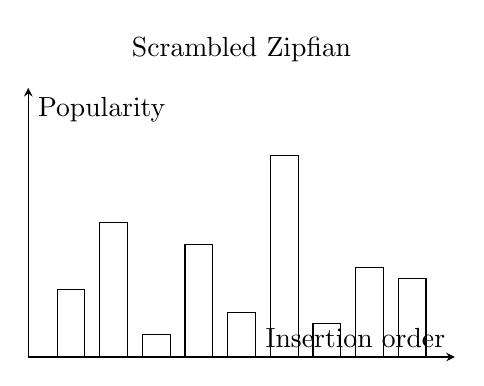
\begin{tikzpicture}
        \begin{axis}[
            width=7cm,
            height=5cm,
            title={Scrambled Zipfian},
            xlabel style={at={(axis description cs:0.5,-0.1)},anchor=north},
            ylabel style={at={(axis description cs:-0.1,.5)},rotate=90,anchor=south},
            xlabel={Insertion order},
            ylabel={Popularity},
            xtick=\empty,
            ytick=\empty,
            axis lines=middle,
            ymin=0, ymax=1.2,
            xmin=0, xmax=10
        ]
        \addplot[ybar,fill=white,draw=black] coordinates {(1,0.3) (2,0.6) (3,0.1) (4,0.5) (5,0.2) (6,0.9) (7,0.15) (8,0.4) (9,0.35)};
        \end{axis}
    \end{tikzpicture}
    \hspace{1cm}
    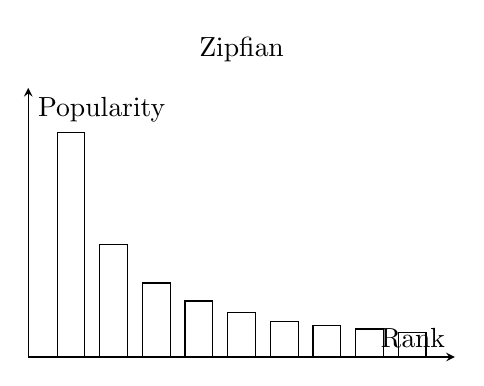
\begin{tikzpicture}
        \begin{axis}[
            width=7cm,
            height=5cm,
            title={Zipfian},
            xlabel style={at={(axis description cs:0.5,-0.1)},anchor=north},
            ylabel style={at={(axis description cs:-0.1,.5)},rotate=90,anchor=south},
            xlabel={Rank},
            ylabel={Popularity},
            xtick=\empty,
            ytick=\empty,
            axis lines=middle,
            ymin=0, ymax=1.2,
            xmin=0, xmax=10
        ]
        \addplot[ybar,fill=white,draw=black] coordinates {(1,1) (2,0.5) (3,0.33) (4,0.25) (5,0.2) (6,0.16) (7,0.14) (8,0.125) (9,0.11)};
        \end{axis}
    \end{tikzpicture}
    \caption{Comparison of Jim Gray's version (right) and the one employed by YCSB (left).}
    \label{fig:zipfian_comparison_ycsb}
\end{figure}

To avoid the issue described earlier, YCSB uses a hashing function to randomly spread the values in support of the distribution and employs an extended domain to reduce collisions \cite{cooperBenchmarkingCloudServing2010}. 

\begin{figure}[h]
  \centering
  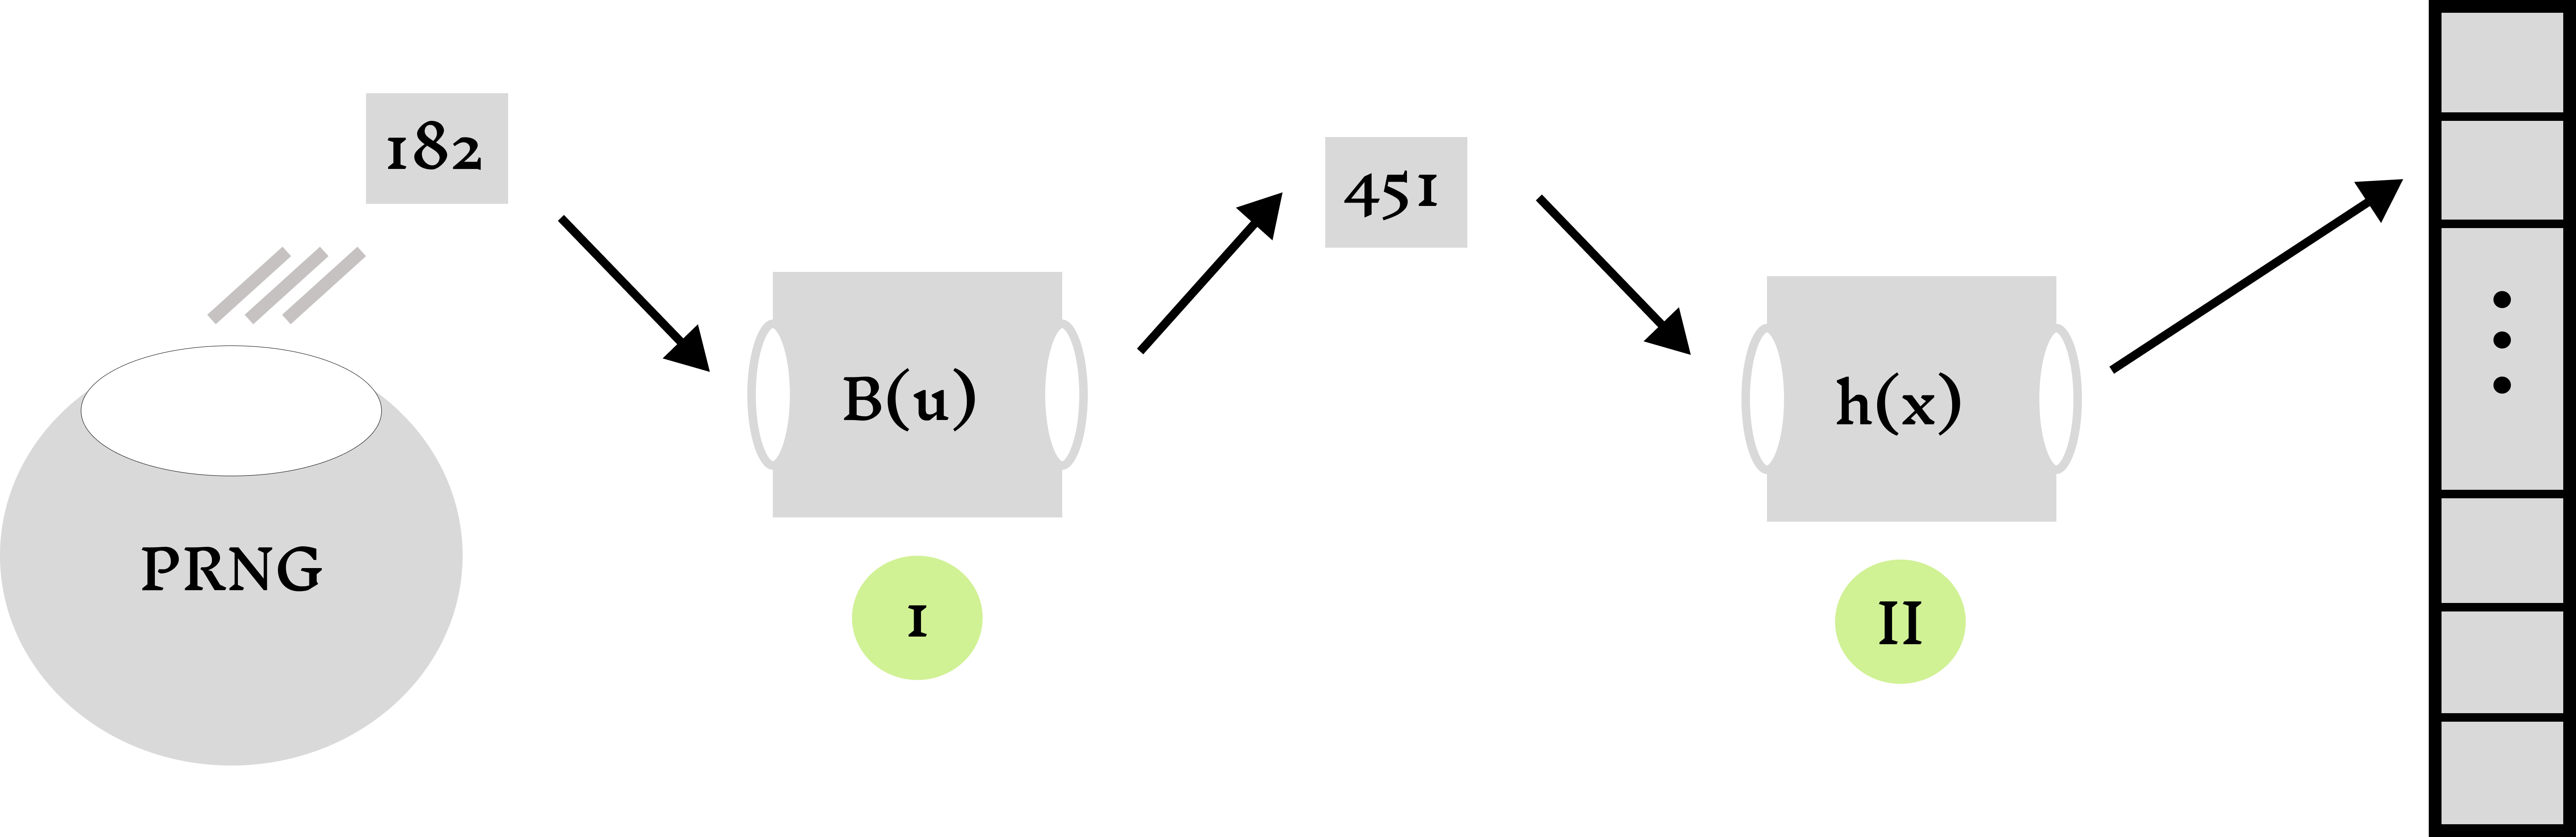
\includegraphics[width=\linewidth]{figures/explanation_ycsb.png}
  \caption{YCSB does sampling by inversion (1) and then hashes the value to spread in in the available range (2)}
  \label{fig:explanation_rej_samp}
\end{figure}

\subsection{Flexible I/O Tester (FIO)}
\ac{FIO} \cite{1FioFlexible} is a benchmarking tool for storage systems. Much like YCSB, its purpose is generating workloads following a certain \textit{access pattern}
to test a storage system. The workloads can vary in type, including sequential or random, and read-only, write-only, or mixed. In the case of \textbf{random I/O}, the user can
change the workload to simulate both asymmetrical and more symmetrical workloads. The underlying distributions include the \textit{Zipfian}, \textit{Normal},
 \textit{Pareto}, and \textit{Uniform} distributions.
 
The algorithm used is also the approximative method due to Jim Gray. As with \ac{YCSB}, the same problem arises with the lexographical ordering of the results, to which
\textit{FIO} resorts to using a hashing function called \textit{lookup3}, in the \textit{Jenkins} collection of hash functions \cite{jenkinsLookup3}.

\subsection{Sysbench}
Sysbench is a benchmarking tool for databases as well as storage systems. It works 
very similarly to YCSB, using multi-threading to strain the system with concurrent accesses. The tool can generate synthetic data
according to different probability distributions, among which the Zipfian distribution.

What sets it apart from the previous is that the variate generation uses a different algorithm. The one employed by Sysbench is based on \textit{Rejection-Inversion sampling} (see Subsection \ref{subsec:rejection_inversion}), 
and the implementation closely follows that from the Apache Commons Math library \cite{MathCommonsMath} under \textit{RejectionInversionZipfSampler}.

\subsection{OLTP-Bench}
The OLTP-Bench \cite{difallahOLTPBenchExtensibleTestbed2013} strives to unify different benchmarks for evaluating a \ac{DBMS}. 
It favors a modular design, enabling very different benchmarks
to be used under a standard interface, which makes it extensible. However, it also has enough benchmarks built-in to be used directly, 
including AuctionMark \cite{AuctionMarkOLTPBenchmark}, \ac{TPC-C}, and \ac{YCSB}. The focus will be on the AuctionMark benchmark,
as it is the one excepting \ac{YCSB}, which generates synthetic data following a Zipfian distribution. The implementation is almost directly based on YCSB, thus not
further differentiated.

\section{Benchmarking Module}
A benchmarking module was developed to evaluate the frameworks. It was written in Python and
allows the user to specify which sample generator to use, as well as the distribution parameters. It is usable from the command line and
includes the following commands: \verb|sample_zipf|, to generate a Zipfian distribution, \verb|accuracy_zipf| to calculate accuracy measures
for one distribution, and \verb|benchmark| to run a specified performance benchmark. It follows a modular design, with the following interfaces:
\textit{SamplerInterface}, responsible for providing a common wrapper interface to all the sampling algorithms; \textit{StorageInterface}, which defines how the 
data is to be stored in memory before processing; and \textit{OutputInterface}, which defines how the data is to be persisted. A UML diagram of the tool is shown in Figure \ref{fig:uml_diagram}.
\begin{figure}
  \centering
  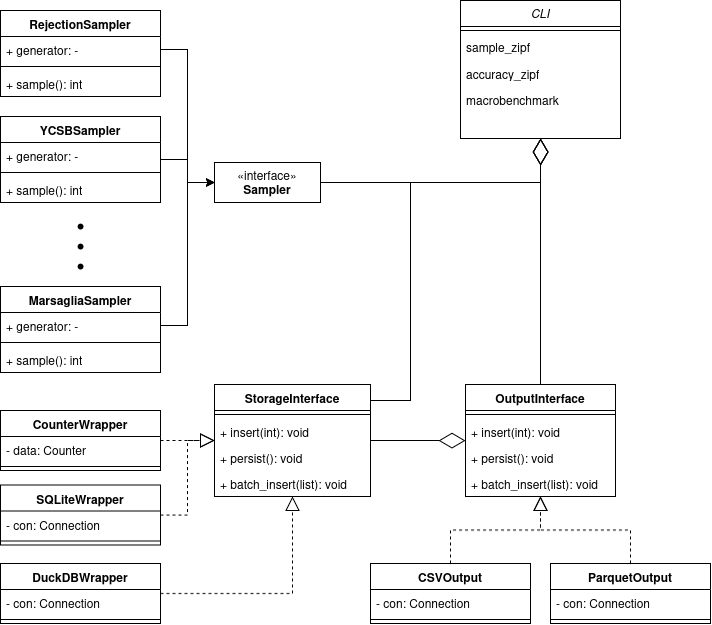
\includegraphics[scale=0.5]{figures/UML.png}
  \caption{UML diagram of the benchmarking module}
  \label{fig:uml_diagram}
\end{figure}

To use the libraries and frameworks described previously, only the necessary code functionality for generating \textit{Zipfian} variates was extracted and packaged
as \textit{shared libraries} and/or \textit{executables}. These were compiled with optimization turned on to ensure a fair comparison.

\subsection{Commands}
To generate a sample, the command \verb|sample_zipf| is used. For example,
\begin{lstlisting}
  sample_zipf --generator sysbench --n 1000 --samples 1000 --skew 1.5 --output csv --storage sqlite --buckets 100
\end{lstlisting}

Running the command will create a CSV file with 1000 samples following a Zipfian distribution with a skew of $1.5$ and a domain from 0 to 1000.
The samples will be stored in memory in a SQLite database with 100 buckets. 

In order to calculate the accuracy measures of the distribution implied by a sample stored in a CSV, the command \verb|accuracy_zipf| is used, as in
\begin{lstlisting}
  accuracy_zipf --input_dir /path/to/csv --skew 1.5 --output_dir /path/to/output
\end{lstlisting}

This method assumes that the directory contains CSV files of results of various sample sizes and domain sizes, belonging to one generator. 
It will then generate 3 CSV files, with columns for domain size and rows for domain sizes - The first one with the \ac{TVD},
the second with the \ac{KS} distance, and the third with the p-value of the \ac{KS} test.
